\documentclass[paper=A4,bibliography=totocnumbered]{scrartcl}
\setkomafont{disposition}{\normalcolor\bfseries} %in KOMA headings are default sans serif, with this patch with serifs see scrguide.pdf, 2010-09-14, page 108
\usepackage[dvipsnames]{xcolor}
\usepackage[latin1]{inputenc} % correct coding for windows e.g. with umlauts
\usepackage[T1]{fontenc}
\usepackage{paralist} % compactenum and compactitem
\usepackage[pdftex]{graphicx} % required to insert figures
\usepackage{listings} % format code
\lstset{escapeinside={<@}{@>}}
\usepackage[margin=10pt,font=small,labelfont=bf,labelsep=endash,singlelinecheck=false,format=plain]{caption} % formatting of captions
\usepackage{booktabs} %for professional tables using \toprule, \midrule, \bottomrule
\usepackage[round]{natbib} % http://merkel.zoneo.net/Latex/natbib.php for author-year citation with round brackets
\usepackage{vmargin} % for margins, especially bottommargin smaller, alternative to DIV=12
\setmarginsrb{35mm}{20mm}{25mm}{15mm}{12pt}{11mm}{0pt}{11mm}

% math packages
\usepackage{amsmath}
\usepackage{amssymb}
\usepackage{centernot}
\usepackage{leftidx}

% set up chapter depths
\newcommand{\subsubsubsection}[1]{\paragraph{#1}\mbox{}\\}
\setcounter{secnumdepth}{4}
\setcounter{tocdepth}{4}
\usepackage{subfig}
\usepackage[hidelinks]{hyperref} % linked pdf, necessarily at the end of preamble!!!

%##########################################################
%###################### Help! #############################
%##########################################################
% 
% Strg+T to comment a block 
% 
% \citet --> Mustermann et al. (2042)
% \citet* --> Mustermann, Musterfrau and Musterkind (2042)
% \citep --> (Mustermann et al. 2042)
% \citep* --> (Mustermann, Musterfrau and Musterkind 2042)
% 
% Insert a picture called xxx.png which is stored in the folder pic as a png
%\begin{figure}
%	\centering
%	\includegraphics[width=13cm]{pic/xxx}
%	\caption[Short Title]{Caption insert here}
%	\label{fig:somelabelname}
%\end{figure}
%
%##########################################################
%########### End Preferences, Begin Document ##############
%##########################################################

%opening
\title{Programming Project 03}
\author{Francel Lamprecht, Christine Robinson, Regina Wehler}
\date{Winter Semester 2018/19}

\begin{document}

\maketitle

\tableofcontents
\clearpage
\section{Introduction}
**REMOVE LATER!This is a dummy sentence that shows how citations work \citep{Adams.2018}.**

Plant phenotyping is a research  area in the plant sciences that focuses on the quantitative measurement of both functional and structural properties of plants. During the last decade plant phenotyping evolved to non-destructive, image-analysis-based phenotyping. This computer driven approach allows the characterization of plants in a high-throughput manner \citep{Walter.2015}.

The focus of this plant phenotyping research project was on the processing, segmentation and classification of Arabidopsis, to gain valuable insight on how the image-analysis-based phenotyping in the life sciences works. 

Arabidopsis is often used as a model plant, as the plant is small in size, with a rapid life cycle of about six weeks \citep{Koornneef.2010}. Arabidopsis is a rosette plant, with the individual leaves being on separate, distinguishable stems. This characteristic of Arabidopsis makes leaf separation from each other less complex.  Given that we were only exploring viable methods in this research area, Arabidopsis was our chosen plant, as it gave us the opportunity to explore with different algorithms in an easier way than what the other given data set, Tobacco, would have allowed us to do. 



\section{Methodology}
The image analysis approach consists of three main steps (figure \ref{fig:pipeline}). First, the input RGB input image is segmented into two classes, plant and background by a trainable Weka segmentation classifier. Second, the binary class output is used to identify single leaf objects by watershed segmentation. The resulting binary mask is utilized to analyze properties of the leaf objects in the single red, green and blue channel, respectively.

\begin{figure}
	\centering
	\subfloat[Input]{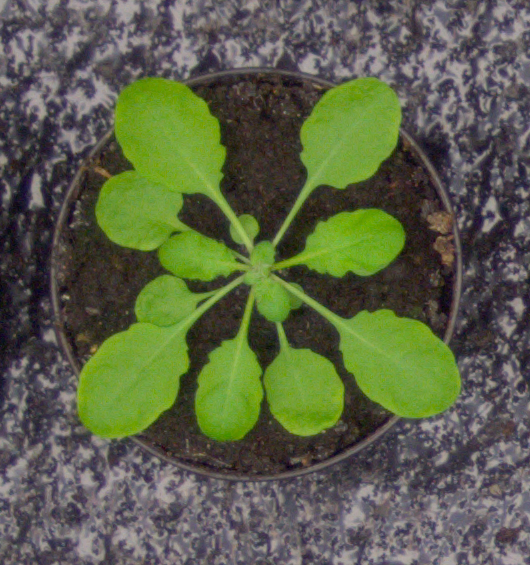
\includegraphics[width=.3\textwidth]{pic/27_rgb}}
	\qquad
	\subfloat[Classification]{
\includegraphics[width=.3\textwidth]{pic/27_class}}
	\qquad
	\subfloat[Watershed]{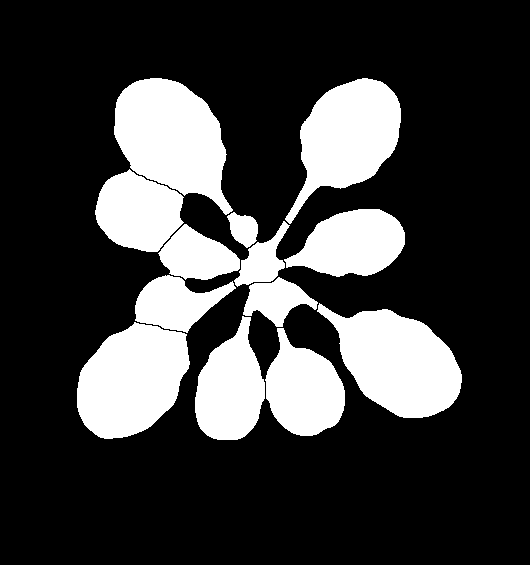
\includegraphics[width=.3\textwidth]{pic/27_watershed}}
	\qquad
	\subfloat[Particle Analysis]{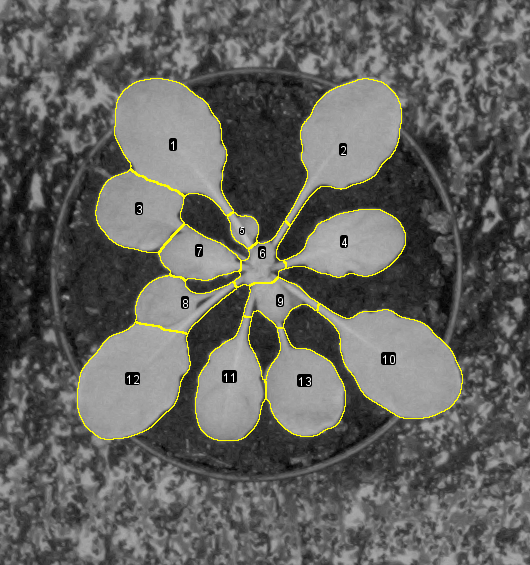
\includegraphics[width=.3\textwidth]{pic/27_greenPA}}
	\caption[Image analysis pipeline]{The analysis of plant leaves is conducted in three steps. The RGB input image (a) is classified into plant and background by a trainable Weka segmentation classifier (b). Single leaf objects are identified by watershed segmentation (c). The binary mask is used to analyze properties in the split red, green and blue channel (d).}
	\label{fig:pipeline}
\end{figure}

\subsection{Segmentation}
The plant is separated from the background with the help of a trainable Weka segmentation classifier, which is available as a plugin for Fiji. Weka provides a GUI to train machine learning algorithms to produce pixel-based segmentations. The user can add traces to classes and train the classifier with those. Afterwards, traces/regions of interest can be adjusted and the classifier can be re-trained to improve classification. Six representative pictures are selected from the 2017 data set for training (plant029, plant145 and plant159 from A1; plant032, plant034 and plant037 from A2). Pictures are chosen to cover the whole range of plant green shades and the range of background characteristics of the given data sets. The Weka Experimenter was used to assess the performance of different machine learning algorithms. Based on these results (table \ref{tab:weka}), FastRandomForest was used as a classifier. By applying the trained classifier to the RGB input images, for each input image a binary classification image is obtained (figure \ref{fig:pipeline}-b). 

\begin{table}[htbp]
	\centering
	\caption{Comparison of classifier performance by Weka Experimenter. The default algorithm parameters were kept.}
	\begin{tabular}{lllllll}
		\toprule
		Algorithm & Percent correct & Precision & Recall & F score & Matthews  & AUC \\
		 & & & & & correlation & \\
		 \midrule
		FastRandomForest & 99.93 & 1.00 & 1.00 & 1.00 & 1.00 & 1.00 \\
		SMO & 92.52 & 0.89 & 0.93 & 0.91 & 0.85 & 0.93 \\
		$k$-nearest Neighbors & 95.38 & 0.95 & 0.93 & 0.94 & 0.90 & 0.95 \\
		RandomSubSpace & 99.85 & 1.00 & 1.00 & 1.00 & 1.00 & 1.00 \\
		Bagging & 99.77 & 1.00 & 1.00 & 1.00 & 1.00 & 1.00 \\
		DesicisonTable & 99.05 & 0.99 & 0.9 & 0.99 & 0.98 & 1.00 \\
		\bottomrule
	\end{tabular}
	\label{tab:weka}
\end{table}

\subsection{Objects Recognition}
A plant consists of leaves that are attached to each other. To be able to analyze leaves individually, they need to be separated. Here, the watershed algorithm was used to separate touching objects. The algorithm first calculates an Euclidean distance map and determines center points as points which are, from a topological view, the ultimate eroded points, As the algorithm's name indicates, this topological map is "flooded" with water and at each collision of two "watersheds", a line separating two objects is drawn. Before watershed was applied, outliers were removed in both classes of the binary image by using the Fiji remove outliers function separately on each class. This function uses a median filter, for which the pixel radius was set to 6 and the threshold was set to 50. The output of the watershed algorithm is the binary image with added watershed lines (figure \ref{fig:pipeline}-c). 

\subsection{Object Analysis}
Particle Analyzer and additional stuff until csv export

\subsection{Explorative Data Analysis}
Everything in Python

\section{Results}


\section{Discussion}
- quality of classification depends on the selection of images for training and on the selection of traces

- need to find a balance between number of labeled pixels and classification accuracy because with increasing number of labeled pixels the reading of the classifier later requires more time

- watershed is working best for circular objects, that's why it sometimes fails on leaves with long stems

- detection and removal of outliers is difficult for very small plants -> with our pipeline we have lost very small plants (pixel number?)


\renewcommand\bibname{References} % necessarily before \bibliography{ref}, but not working in preamble
\bibliographystyle{apalike} % for references chapter
\bibliography{ref}

\end{document}
